\documentclass[10pt]{article}
\usepackage[T2A]{fontenc}
\usepackage[utf8]{inputenc}
\usepackage[english,russian]{babel}
\usepackage{amsfonts, amssymb, amsmath, amsthm}
\usepackage{graphicx}
\usepackage{subcaption}
\usepackage[font=small]{caption}
\usepackage{wrapfig}
\usepackage{enumitem}
\usepackage{tabto}
\usepackage{float}
\usepackage{algorithm}
\usepackage{algpseudocode}
\setlist{noitemsep}
\usepackage[left=2cm,right=2cm,top=2cm,bottom=2cm]{geometry}

\renewcommand{\leq}{\leqslant}
\renewcommand{\geq}{\geqslant}
\renewcommand{\phi}{\varphi}
\newcommand{\R}{\mathbb{R}}
\newcommand{\E}{\mathbf{E}}
\renewcommand{\C}{\mathcal{C}}
\newcommand{\bF}{\bar{\mathcal{F}}}
\newcommand{\F}{\mathcal{F}}
\newcommand{\cY}{\check{Y}}
\newcommand{\wY}{\widetilde{Y}}
\newcommand{\wDelta}{\widetilde{\Delta}}
\renewcommand{\wp}{\widetilde{p}}
\newcommand{\wq}{\widetilde{q}}
\newcommand{\wf}{\widetilde{f}}
\newcommand{\wrho}{\widetilde{\rho}}
\newcommand{\hq}{\widehat{q}}
\newcommand{\eps}{\varepsilon}

\newtheorem{theorem}{Теорема}
\newtheorem{proposition}{Утверждение}
\newtheorem{definition}{Определение}
\newtheorem{remark}{Замечание}
\newtheorem{proving}{Доказательство}
\DeclareMathOperator{\diag}{diag}
\DeclareMathOperator*{\argmin}{arg\,min}

\title{Обучение без учителя. Разделение смеси распределений. Кластеризация. Тематическое обучение (Probabilistic LSA). }
\author{Смирнов~И, Михайлов~Д.}


\begin{document}
\maketitle
	
	
\section{Обучение без учителя}

Обучение без учителя - это один из способов машинного обучения, при котором испытуемая система обучается выполнять поставленную задачу без вмешательства со стороны экспериментатора.  Как правило, это пригодно только для задач, в которых известны описания множества объектов (обучающей выборки), и требуется обнаружить внутренние взаимосвязи, зависимости, закономерности, существующие между объектами

Обучение без учителя становится формально поставленной задачей только в случае, если можно написать функцию правдоподобия

\section{Кластеризация}

\subsection{Введение в задачу кластеризации}

Задача кластеризации заключается в том чтобы выполнить разбиение индивидов на кластеры на основе их сходства друг с другом (близость относительно выбранной метрики), при этом сами кластеры или их количество, как правило, заранее не известны. Кластеры строятся так, что характеристики для объектов внутри одного кластера близки, а характеристик объектов из разных кластеров сильно отличаются.

\subsection{Формальное описание задачи класстеризации}

Пусть имеется подмножество $\pmb X \subset \mathbb{R}^{p}$, которое будем называть
пространством объектов, выборка $\pmb X^{n} = \{\pmb x_1, \dots, \pmb x_{n}\}$, где $\pmb x_{i} $ --- индивиды, определяемые вектором признаков, $C$ --- множество кластеров. Задача состоит в том чтобы найти такую функцию $a: X \rightarrow Y$, которая разбила бы выборку на непересекающиеся кластеры $\pmb X^{n}= \bigcup_{j = 1}^{k} C_{j}, \  C_{i} \bigcap C_{j} = \emptyset$, таким образом, чтобы объекты одного кластера были близки по функции расстояния между объектами $\rho :  \mathbb{R}^{p} \times  \mathbb{R}^{p} \rightarrow [0,\infty)$ и существенно отличались для объектов разных кластеров.


Не существует <<истинных>> или <<лучших>> определений для кластера. Что понимать под кластером должно быть определено исследователем, который применяет методы кластеризации. Как правило, для этого нужно определить характеристики кластера в отношении размера и формы, а также предполагаемых различий между кластерами.

Общая схема процесса кластеризации данных включает в себя: 
\begin{itemize}
	\item определение меры сходства;
	\item разбиение множества объектов на кластеры;
	\item оценку качества кластеризации;
	\item интерпретацию результатов.
\end{itemize}
	
Решение задачи кластеризации принципиально неоднозначно, так как число кластеров, как правило, не известно заранее, к тому же результат кластеризации сильно зависит от метрики $\rho$, выбор которой также не однозначен.

\subsection{Подходы к решению задачи кластеризации}

\subsubsection{EM - алгоритм для model-based подхода}

Один из вариантов формализовать задачу кластеризации это сделать предположение о статистическом распределении данных. Затем задача будет состоять в поиске параметров этого распределения. Предположим, что модель данных состоит из $k$ смеси распределений. Пусть $\omega_{1}\ldots \omega_{k}$ --- априорные вероятности появления объектов из соответствующих кластеров, $p_{1}(x)\ldots p_{k}(x)$ --- плотности распределения признаков внутри кластеров. Тогда плотность распределения сразу для всех кластеров равна взвешенной сумме плотностей по каждому кластеру:
$$
p(x) = \sum\limits_{i=1}^k \omega_{i} p_{i}(x).
$$
Поставим задачу разделения смеси распределений, оценим по выборке $\omega_{1}\ldots \omega_{k}$ и $p_{1}(x)\ldots p_{k}(x)$. Это позволит оценить вероятность принадлежности индивида к разным кластерам и решить к какому кластеру его отнести. Часто рассматриваются случаи когда распределение смеси принадлежат одному семейству распределений, например нормальному, но с разным набором параметров для каждого из кластеров. 
$$
p_{i}(x) = \varphi(\theta_{i}; x)
$$
Согласно методу максимального правдоподобия 
$$
\omega, \theta = \underset{\omega, \theta}{\text{argmax}} \sum\limits_{i=1}^n \ln{p(x_{i})}  =  \underset{\omega, \theta}{\text{argmax}} \sum\limits_{i=1}^n \ln  \sum\limits_{j=1}^k \omega_{j}  \varphi(\theta_{j}; x_{i})
$$
Максимизация логарифма суммы достаточно сложна, поэтому задача не решается напрямую с помощью метода максимума правдоподобия. Для максимизации логарифма функции правдоподобия применяется EM-алгоритм. Это итеративный алгоритм, состоящий из двух шагов, в котором на первом шаге задаются какие-нибудь значения параметров, а затем с каждой итерацией эти параметры уточняются.

\textbf{E - шаг.}

В начале работы алгоритма задаём значения параметров $\omega, \theta = (\omega_{1}\ldots, \omega_{k};\theta_{1}\ldots \theta_{k})$, и подставляя их рассчитываем скрытые переменные. Скрытые переменные $h_{ij} = P(\theta_{j}|x_{i})$ --- это вероятность того, что индивид $x_{i}$ принадлежит $j$ смеси. Найдем скрытые переменные по формуле Байеса:
$$
h_{ij} = \frac{ \omega_{j} \varphi(\theta_{j}; x_{i})}{\sum\limits_{s=1}^k \omega_{s}  \varphi(\theta_{s}; x_{i})}.
$$
Для любого индивида $\sum\limits_{j=1}^k h_{ij} = 1.$

\textbf{M - шаг.}

На этом шаге будут рассчитываться значения параметров, которые мы ищем, используя скрытые параметры, полученные на предыдущем шаге. Решение методом Лагрнажа для максимизации (\ref{maxlog}) (c ограничением $\sum\limits_{j=1}^k\omega_{j}=~1$) даёт оценку для параметров:
$$
\omega_{j} = \frac{1}{n} \sum\limits_{i=1}^n h_{ij}
$$
$$
\theta_{j} = \underset{\theta}{\text{argmax}} \sum\limits_{i=1}^n h_{ij} \ln{\varphi(\theta; x_{i})}
$$
Таким образом, параметры будут уточняться на каждом шаге.

Если сделать предположение о том что классы принадлежат семейству нормальных распределений, то параметрами модели являются математическое ожидание и ковариационная матрица. Если не делать никаких предположений о ковариациях использование общей модели может быть весьма затруднительно, проблема заключается в большом количестве параметров, которые необходимо оценить. Ковариационные матрицы описывают геометрические характеристики кластеров, а именно объем, форму и ориентацию кластера. Общая модель предполагает, что все эти геометрические характеристики различны для каждого кластера. Однако, оценка плотности смеси, состоящей из кластеров одинаковой формы или ориентации, намного проще. Поэтому, сделав предположения о ковариационных матрицах, можно существенно облегчить задачу.

\subsubsection{Алгоритм k-средних (k-means)}
	Метод k-means осуществляет декомпозицию набора данных, состоящего из $n$ наблюдений, на $k$ кластеров с заранее неизвестными параметрами. При этом выполняется поиск центроидов - максимально удаленных друг от друга центров сгущений точек $C_k$ с минимальным разбросом внутри каждого кластера. 
	
	В качестве меры близости выбрано евклидово расстояние: $$ d(\pmb x_{i}, \pmb x_{i'}) = \sum\limits_{j=1}^p (x_{ij} - x_{i'j})^{2} = \| \pmb x_{i} - \pmb x_{i'} \|^{2}. $$
	
	Основная идея алгоритма заключается в минимизации меры близости между индивидами внутри одного кластера: $$ \underset{C_{1},\ldots, C_{k}}\min \left\{ \sum\limits_{l=1}^k \frac{1}{|C_{l}|} \sum\limits_{i,i' \in C_{l}} \| \pmb x_{i} - \pmb x_{i'} \|^{2} \right\}. $$
	
	
	\subsubsection*{Алгоритм}
	
	\begin{enumerate}
		\item Выбираем начальное приближение центров кластеров $\pmb \mu_{1},\ldots, \pmb \mu_{k}$ случайным образом; 
		\item Соотносим каждый объект к ближайшему центру (аналог E-шага) $$C(i) = \underset{0 \leq j \leq k}{\text{argmin}} \|\pmb x_{i} - \pmb \mu_{j} \|^{2};$$
		\item Для каждого кластера $C_{j}$ пересчитываем центры $\pmb \mu_{j}$ как выборочное среднее индивидов, которые были отнесены к этому кластеру (аналог M-шага);
		\item  Повторяем шаги 2 и 3 пока принадлежность кластерам не перестанет изменяться.
	\end{enumerate}
	
	Иными словами, делаем следующее: инициализируем центры, затем разделяем индивиды по ближайшему центру кластера, перевычисляем каждый из центров, и если ничего не изменилось, останавливаемся, если изменилось, то повторяем.
	
	\subsubsection*{Сложность и возможные оптимизации}
	
	Средняя сложность определяется как $O(k n T)$, где $k$ --- количество кластеров, $n$ --- количество индивидов, а $T$ --- количество итераций до сходимости.
	
	Сложность в наихудшем случае определяется как $O(n^{k+2/p})$, где $n$ --- количество индивидов, $p$ --- количество признаков.
	
	На практике алгоритм $k$-средних очень быстр (один из самых быстрых доступных алгоритмов кластеризации), но он попадает в локальные минимумы. Вот почему может быть полезно перезапустить его несколько раз.
	
	При больших $n$ целесообразно использовать модификацию MiniBatchKMean, который выполняет обновления позиций центров с помощью мини-пакетов вместо всей выборки.
	
	При  больших $p$ целесообразно уменьшить размерность простанства признаков с помощью АГК.
	
	\subsubsection*{k-means и его связь с EM - алгоритмом}
	
	
	 Алгоритм k-средних является частным случаем для гауссовой смеси распределения с диагональными ковариационными матрицами, у которых одинаковые значения на диагоналях.
	
	В таком случае:
	\begin{itemize}
		\item На Е-шаге мы не считаем вероятности $g_{ij}$ принадлежности $i$-го объекта $j$-ому кластеру, а приписываем каждый объект одному кластеру (вероятность принадлежности будет равна 0 или 1);
		\item Форма кластеров не настраивается: они все являются сферическими.
	\end{itemize}
	
	\subsubsection*{Достоинства и недостатки}
	
	\textbf{Достоинства:}
	\begin{itemize} 
		\item Простота реализации
		\item Алгоритм очень гибкий 
		\item Cуществует множество различных модификаций этого алгоритма
	\end{itemize}
	
	\textbf{Недостатки:} 
	\begin{itemize}
		\item Кластеризация очень сильно зависит от начального приближения\\
		\textit{Выгодно брать максимально удаленные друг от друга центры. Неудачный выбор центров может привести к плохому результату кластеризации. Для решения этой проблемы можно провести кластеризацию с несколькими начальными приближениями и выбрать лучший вариант.
		Также на практике работает следующая эвристика (K-means++): первый центр выбираем случайно из равномерного распределения на точках выборки, а каждый следующий центр выбираем из случайного распределения на объектах выборки, в котором вероятность выбрать объект пропорциональна квадрату расстояния от него до ближайшего к нему центра кластера.}
		
		\item Кластеризация может быть неадекватной, если изначально было выбрано неверное число кластеров 
		\item Необходимость самостоятельно задавать число кластеров\\ 
		\textit{Подбирать число кластеров можно с помощью коэффицента силуэта, либо использовать метод “локтя” (elbow method), который рассматривает характер изменения внутригруппового разброса с увеличением числа групп $k$. На каком-то этапе снижение этой дисперсии замедляется --- на графике это происходит в точке, называемой “локтем” (аналогично “каменистой осыпи” для анализа главных компонент).}
		
		\item Форма кластеров только сферическая
	\end{itemize}

\subsubsection{Иерархическая кластеризация}
	
	Методы иерархической кластеризации основываются на двух идеях:
	\begin{itemize}
		\item агломерации (AGNES) --- последовательное объединение индивидуальных объектов или их групп во все более крупные подмножества
		\item разбиении (DIANA) ---  начинается с корня и на каждом шаге делит образующие группы по степени их гетерогенности
	\end{itemize}

	Более распространены агломеративные алгоритмы, общий вид которых приведён ниже. 

	
	\subsubsection*{Алгоритм агломеративной иерархической кластеризации}
	\begin{enumerate}
		\item Одноэлементые кластеры: $$C_1 = \left\{\{\pmb x_1\}, \dots, \{\pmb x_n\}\right\}; \; R_1 = 0$$ $$\forall\, i \neq j \text{ вычислить } R(\{\pmb x_i\}, \{\pmb x_j\})$$ 
		\item для всех $t = 2, \dots, n$ ($t$ $-$ номер итерации) 
		\item найти в $C_{t-1}$ два ближайших кластера: $$(U, V) = \arg \min_{U \neq V} R(U, V); R_t=R(U, V);$$
		\item слить их в один кластер: $$W = U \cup V; \; C_t = C_{t-1} \cup W \backslash \{U, V\}$$ 
		\item для всех $S \in C_t \backslash W $ 
		\item вычислить расстояние $R(W, S)$ по формуле Ланса-Уильямса.
	\end{enumerate}

В начальный момент времени каждый объект содержится в собственном кластере. Далее происходит итеративный процесс слияния двух ближайших кластеров до тех пор, пока все кластеры не объединятся в один или не будет найдено необходимое число кластеров. На каждом шаге необходимо уметь вычислять расстояние между кластерами и пересчитывать расстояние между новыми кластерами. 

Расстояние между одноэлементными кластерами определяется через расстояние между объектами: $R(\{x\}, \{y\})= \rho(x,y)$. То есть сначала нужно задать, как мы будем измерять расстояние между точками. Например, это могут быть
\begin{itemize}
	\item Евклидово расстояние: $\rho(x,y) = \sqrt{\sum_i (x_i - y_i)^2}$.
	\item Расстояние городских кварталов (манхэттенское расстояние):  $\rho(x,y) = \sum_i |x_i - y_i|$.
	\item Расстояние Чебышёва: $\rho(x,y) = \max_i |x_i - y_i|$.
\end{itemize}
Важно либо исходно стандартизовать признаки, либо измерять расстояние
специальным образом (использовать расстояние Махаланобиса вместо обычного евклидового, если есть предположения о форме распределения точек внутри кластера).


Для вычисления же расстояния $R(U, V)$ между кластерами $U$ и $V$ на практике используются различные функции в зависимости от специфики задачи.
Изначально было придумано множество различных способов определить такие расстояния, но оказалось, что практически все разумные, являются частным случаем \textbf{формулы Ланса-Уильямса}, которая позволяет обобщить большинство способов определить расстояние между кластерами $ R(W, S),\; W = U \cup V,\, U,\, V,\, S \subset X, $ зная расстояния $R(U, S)$, $R(V, S)$, $R(U, V)$: 
	
	$$ R(W, S) = \alpha_{U} R(U, S) + \alpha_{V} R(V, S) + \beta R(U, V) + \gamma|R(U, S) - R(V, S)|,$$
	
	где $\alpha_{U}$, $\alpha_{V}$, $\beta$, $\gamma$ --- числовые параметры.
	

Ниже приведены некоторые способы определения расстояний явно и соответствующие им коэффициенты для формулы Ланса-Уильямса. 
\begin{itemize}
	\item Расстояние ближнего соседа (single linkage clustering) --- расстояние между кластерами оценивается как минимальное из дистанций между парами объектов, один из которых входит в первый кластер, а другой - во второй:
	$$R^{\text{б}}(W, S) = \min_{w \in W, s \in S} \rho(w, s); \quad \alpha_U=\alpha_V=1/2,\enspace \beta=0,\enspace \gamma=-1/2;$$
	\item Расстояние дальнего соседа (complete linkage clustering) --- вычисляется расстояние между наиболее удаленными объектами:
	$$R^{\text{д}}(W, S) = \max_{w \in W, s \in S} \rho(w, s); \quad \alpha_U=\alpha_V=1/2,\enspace \beta=0,\enspace \gamma=1/2;$$
	\item Среднее расстояние (average linkage clustering) --- на каждом следующем шаге объединяются два ближайших кластера, рассчитывая среднюю арифметическую дистанцию между всеми парами объектов:
	$$R^{\text{с}}(W, S) = \frac{1}{ |W| |S| } \sum_{w \in W} \sum_{s \in S} \rho(w, s); \quad \alpha_U=\frac{|U|}{|W|},\enspace \alpha_V=\frac{|V|}{|W|},\enspace \beta=\gamma=0;$$
	
	\item Расстояние между центрами:
	$$R^{\text{ц}}(W, S) = \rho^2 \left( \sum_{w \in W} \frac{w}{|W|}, \sum_{s \in S} \frac{s}{|S|}\right); \quad
	\alpha_U=\frac{|U|}{|W|},\enspace \alpha_V=\frac{|V|}{|W|},\enspace \beta= -\alpha_U \,\alpha_V,\enspace \gamma=0;$$
	\item Расстояние Уорда (метод минимума дисперсии Уорда):
	$$R^{\text{ц}}(W, S) = \frac{|S| |W|}{|S| + |W|} \rho^2 \left( \sum_{w \in W} \frac{w}{|W|}, \sum_{s \in S} \frac{s}{|S|}\right);$$  
	$$\alpha_U=\frac{|S|+|U|}{|S|+|W|},\enspace \alpha_V=\frac{|S|+|V|}{|S|+|W|},\enspace \beta= -\frac{|S|}{|S|+|W|},\enspace \gamma=0;$$
	
	\item Гибкое расстояние: $$\scalebox{0.9}{$\alpha_U=\alpha_V=\frac{1-\beta}{2},\enspace \beta<1 \;(-0.25),\enspace \gamma=0$}.$$
\end{itemize}.


\subsubsection*{Визуализация кластерной структуры}
Результатом работы иерархического алгоритма является \textbf{дендрограмма} 
--- древовидный график расстояний, при которых произошло слияние кластеров на каждом шаге.
В узлах дерева находятся подмножества объектов. При этом на каждом ярусе дерева множество объектов из всех узлов составляет исходное множество объектов. Объединение узлов между ярусами соответствует слиянию двух кластеров. При этом длина ребра соответствует расстоянию между кластерами. Введем обозначение $R_t$ --- расстояние между кластерами, выбранными на шаге $t$ для объединения. Дендрограмма позволяет представлять зависимости между множеством объектов с любым числом заданных характеристик на двумерном графике, где по одной из осей откладываются все объекты, а по другой --- расстояние $R_t$. Если не накладывать на это расстояние никаких ограничений, то дендрограмма будет иметь большое число самопересечений и изображение перестанет быть наглядным. Чтобы любой кластер мог быть представлен в виде непрерывного отрезка на оси объектов и ребра не пересекались, необходимо наложить ограничение монотонности на $R_t$.

\begin{definition}
	Функция расстояния $R$ является монотонной, если на каждом следующем шаге расстояние между кластерами не уменьшается: $R_1 \leq R_2 \leq \dots \leq R_m$
\end{definition}

Вторым желательным свойством является свойство растяжения. Кластеризация называется сжимающей, если $R_t \leq \rho(\mu_U, \mu_V), \forall t$ и называется растягивающей, 
если $R_t \geq \rho(\mu_U, \mu_V), \forall t$.
При выборе сжимающих расстояний объекты с каждым шагом всё больше слипаются друг с другом.
Свойство растяжения же позволяет лучше отделять кластеры друг от друга. 
Однако, при этом расстояние не должно быть сильно растягивающим, иначе объекты удалятся друг от друга настолько, что появится много лишних кластеров. 
В качестве меры растяжения рассматривается отношение расстояния между кластерами к расстоянию между центрами кластеров. 
Относительно приведённых свойств самыми оптимальными оказываются расстояние Уорда и гибкое расстояние, 
а расстояние между центрами оказывается самым плохим, поскольку оно единственное не является монотонным. 
При этом гибкое расстояние оказывается сжимающим при $\beta >0$ и растягивающим при $\beta <0$. 

Для определения числа кластеров находится интервал максимальной длины $|R_{t+1}-R_t|$ (длинная ветка у дерева). В качестве итоговых кластеров выдаются кластеры, полученные на шаге $t$. Однако, когда число кластеров заранее неизвестно и объектов в выборке не очень много, бывает полезно изучить дендрограмму целиком.

\begin{figure}[H]
	\centering
	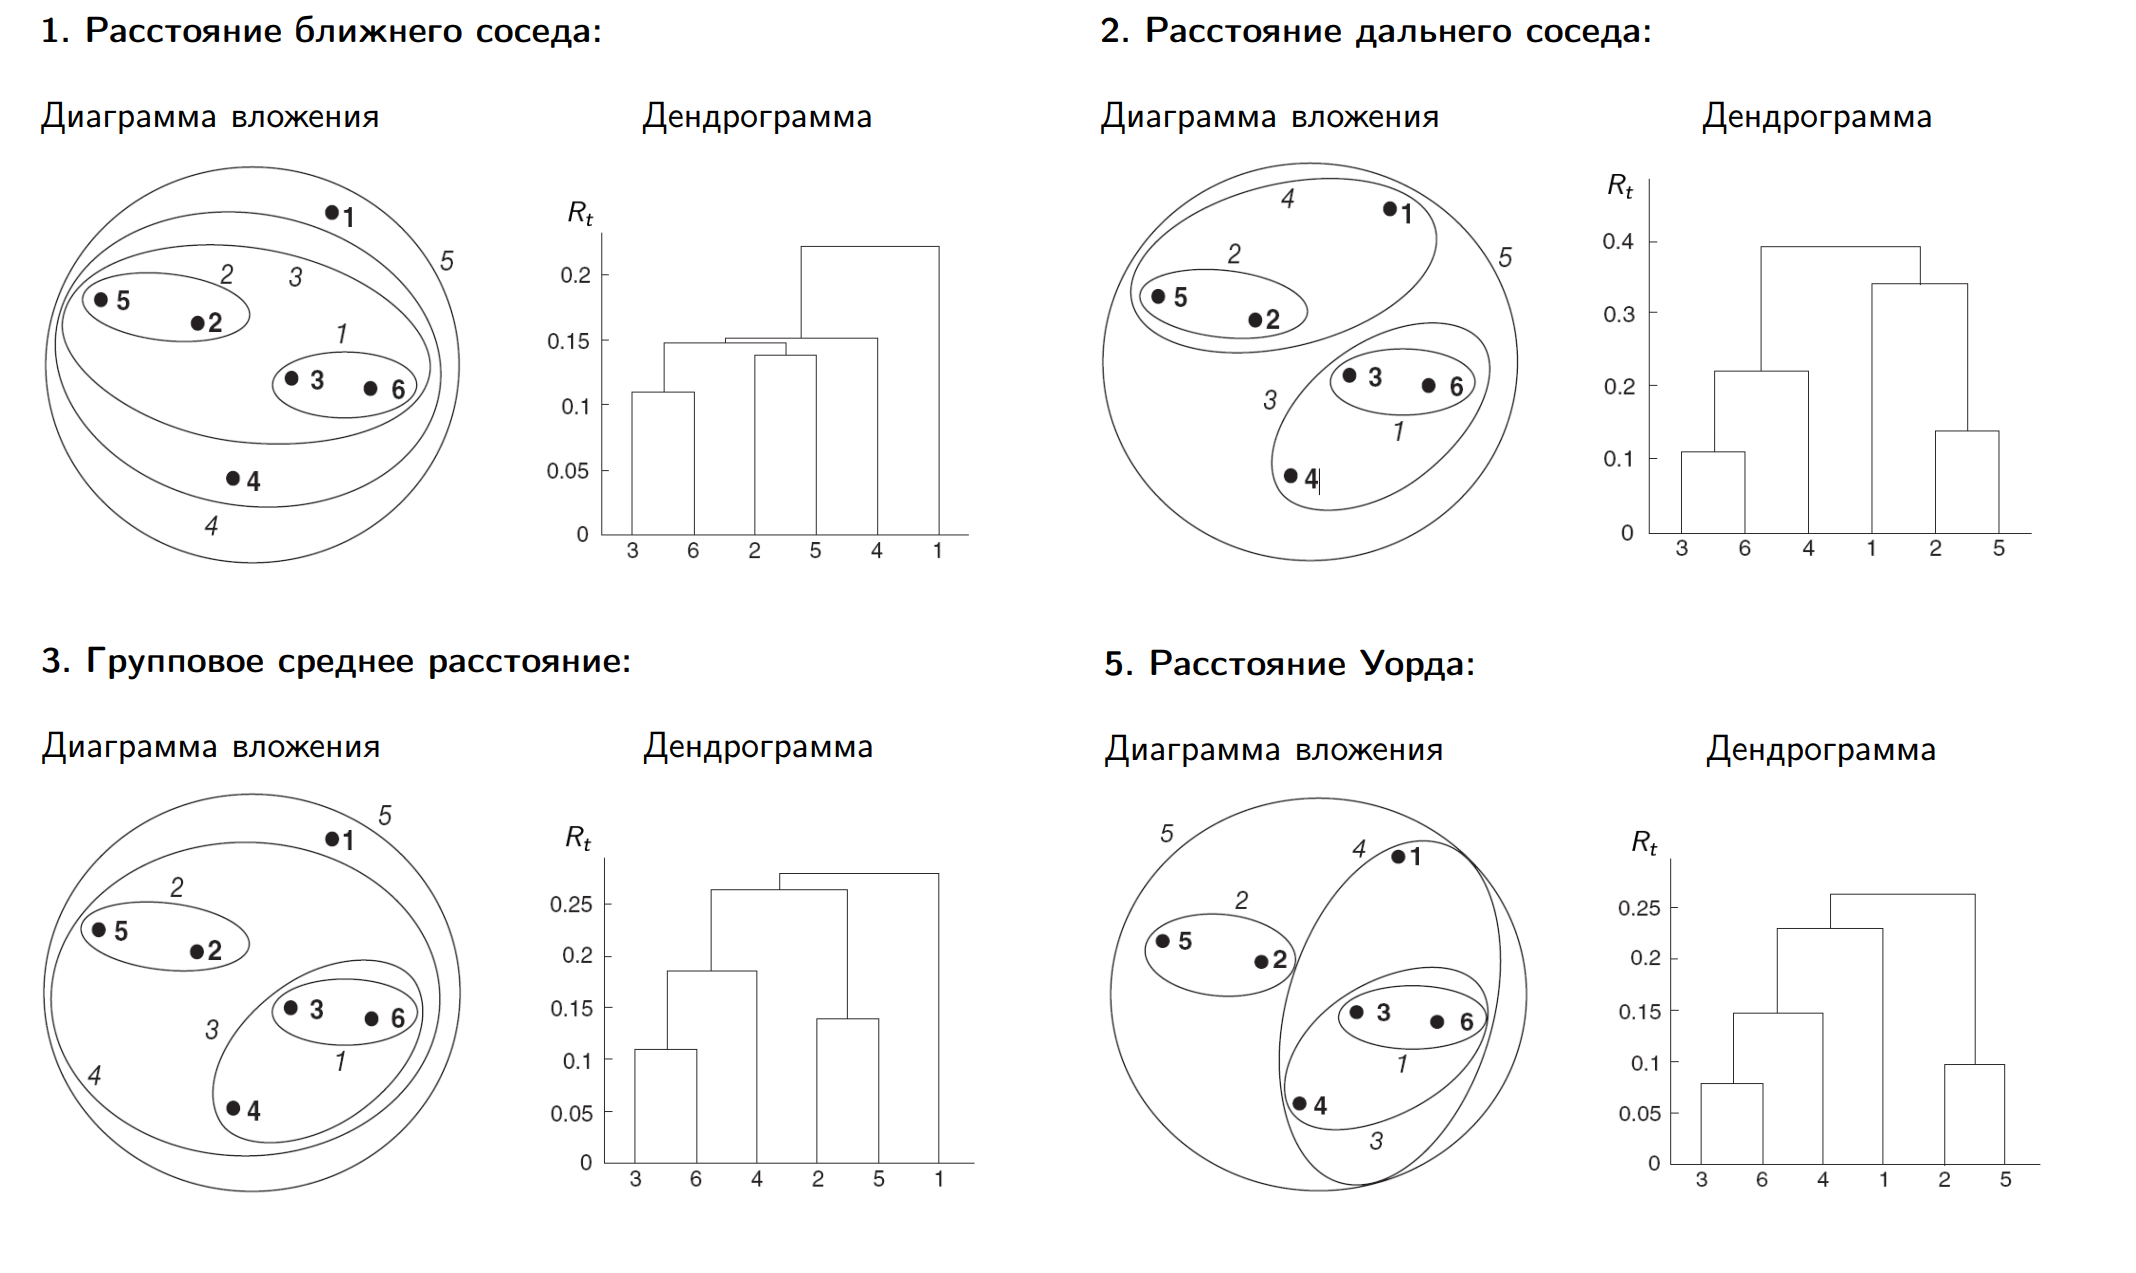
\includegraphics[scale=0.2]{hier.png}
	\caption{Дендрограммы при выборе различных расстояний.}
\end{figure}


\subsubsection*{Плюсы и минусы}
\textbf{Достоинства:}
\begin{itemize}
	\item В качестве результата можно получить дендрограмму, которая может представлять самостоятельный интерес. 
	\item Форма кластеров может быть произвольной.
	\item Количество кластеров можно определить по дендрограмме.
\end{itemize}

\textbf{Недостатки:}
\begin{itemize}
	\item Необходимость подбирать одно из множества различных расстояний.
	\item Отсутствие модели в задаче не позволяет однозначно предпочесть одно разделение на кластеры другому.	
\end{itemize}

\subsubsection{Алгоритм DBSCAN}

\textbf{DBSCAN} (Density-based spatial clustering of applications with noise) --- это эвристический алгоритм кластеризации, который предложили Маритин Эстер, Ганс-Петер Кригель, Ёрг Сандер и Сяовэй Су в 1996. Это алгоритм кластеризации, основанный на плотности --- алгоритм группирует вместе те объекты, которые тесно расположены, помечая как выбросы объекты, которые находятся в областях с малой плотностью.

	
В этом алгоритме рассматривается для каждого объекта $\pmb x \in U$ его $\varepsilon$-окрестность $U_\varepsilon (\pmb x) = \{\pmb u \in U : \rho(\pmb x , \pmb u ) \leq \varepsilon\}$.
	
Каждый объект может быть одного из трёх типов:
	\begin{itemize}
		\item корневой: имеет плотную окрестность $|U_\varepsilon (\pmb x)| \geq m$ 
		\item граничный: не корневой, но находится в окрестности корневого 
		\item выброс: не корневой и не граничный. 
	\end{itemize}

\begin{figure}[H]
	\begin{center}
		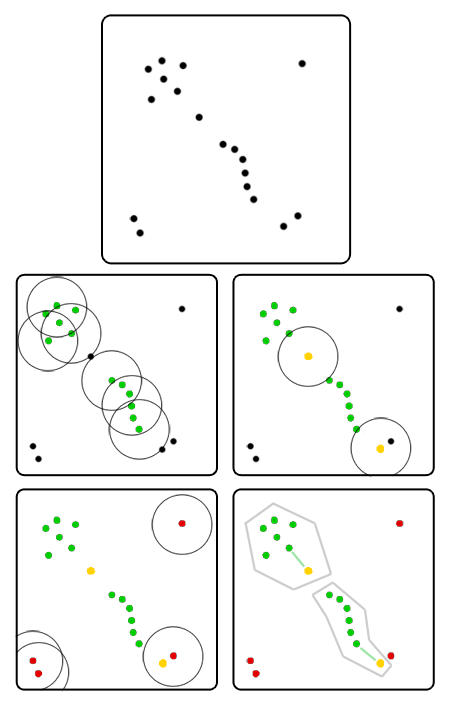
\includegraphics[scale = 1.5]{dbscan.png}
		\caption{Иллюстрация к алгоритму DBSCAN. На рисунке зелёным отмечены корневые объекты, жёлтым~---~граничные и красным~---~шумовые.}
	\end{center}
\end{figure}
	
Корневые объекты находящиеся в $\eps$-окрестности друг друга объединяются в один кластер. Граничные объекты относятся к тому кластеру, к какому относится корневой
объект, в $\eps$-окрестности которого лежит данный граничный объект. Таким образом, в итоге получается разделение всех объектов на кластеры и шумовые объекты.

\subsubsection*{Алгоритм}
	
\textbf{Вход:} выборка $\pmb X^{n} = \{\pmb x_1, \dots, \pmb x_{n}\}$, параметры $\varepsilon$ и $m$;
	
\textbf{Выход:} разбиение выборки на кластеры и шумовые выбросы;
\begin{enumerate}
		\item $U=X^n$, $a=0$; 
		\item \textbf{Пока} есть некластеризованные точки, т.е. $U \neq \varnothing$; 
		\item \quad взять случайную точку $\pmb x \in U$; 
		\item \quad \textbf{если} $|U_\varepsilon (\pmb x)| < m$, \textbf{то} 
		\item \quad \quad пометить $\pmb x$ как шумовой; 
		\item \quad \textbf{иначе} 
		\item \quad \quad создать новый кластер: $K=U_\varepsilon (\pmb x)$; $a = a + 1$; 
		\item \quad \quad \textbf{для всех} $\pmb x' \in K$ 
		\item \quad \quad \quad \textbf{если} $|U_\varepsilon (\pmb x')| \geq m$ \textbf{то} $K=K \cup U_\varepsilon(\pmb x')$; 
		\item \quad \quad \quad \textbf{иначе} пометить $\pmb x'$ как граничный элемент $K$; 
		\item \quad \quad соотнести объект классу $a$ для всех $\pmb x' \in K$; 
		\item \quad \quad $U=U \setminus K$ 
\end{enumerate}

\subsubsection*{Плюсы и минусы}
\textbf{Достоинства:} 
\begin{itemize}
	\item Относительно быстрая кластеризация больших данных (от $O(n \ln n)$ до $O(n^2)$ в зависимости от реализации); 
	\item Позволяет обрабатыват кластеры произвольной формы (в том числе протяжённые ленты, концентрические гиперсферы); 
	\item Помимо деления на кластеры выдаёт ещё и разметку шумовых объектов; 
	\item Cам определяет количество кластеров (по модулю задания других гиперпараметров);
	\item Хорошо поддаётся модифицированию (существуют реализации, скрещенные с k-means, например). 
\end{itemize}

\textbf{Недостатки:}\\ 
	Алгоритм может неадекватно обрабатывать сильные вариации плотности данных внутри кластера, проёмы и шумовые мосты между кластерами.
	То есть метод не способен соединять кластеры через проёмы, и, наоборот, связывает явно различные кластеры через плотно населённые перемычки. Проблема особенно актуальна для данных большой размерности, так как чем больше $p$, тем больше мест, где могут случайно возникнуть проёмы или мосты. 

\subsection{Функционалы качества кластеризации}

Задачу кластеризации можно ставить как задачу дискретной оптимизации:
приписать номера кластеров объектам так, чтобы значение выбранного функционала качества приняло наилучшее значение.
Существует много разновидностей функционалов качества кластеризации, но нет <<самого правильного>>. По сути дела, каждый метод кластеризации можно рассматривать как точный или приближённый алгоритм поиска оптимума некоторого функционала.	
Исходя из начальной постановки задачи <<меньше расстояние внутри кластеров --- больше снаружи>>, естественно выбрать среднее внутрикластерное и среднее межкластерное расстояние.

\subsubsection{Среднее внутрикластерное расстояние}
$$F_0 = \frac{\sum_{i < j}\mathbf{I}_{\{y_i = y_j\}}\rho(\pmb x_i, \pmb x_j)}{\sum_{i < j}\mathbf{I}_{\{y_i = y_j\}}},$$ 

Решая задачу кластеризации, мы хотим по возможности получать как можно более кучные кластеры, то есть минимизировать $F_0$.

\subsubsection{Среднее межкластерное расстояние}

$$F_1 = \frac{\sum_{i < j}\mathbf{I}_{\{y_i \neq y_j\}}\rho(\pmb x_i, \pmb x_j)}{\sum_{i < j}\mathbf{I}_{\{y_i \neq y_j\}}}.$$

Среднее межкластерное расстояние, напротив, нужно максимизировать, то есть целесообразно выделять в разные кластеры наиболее удалённые друг от друга объекты.

Имеет смысл вычислять отношение пары функционалов, чтобы учесть как внутрикластерные, так и межкластерные расстояния: $F_0/F_1 \rightarrow min$.


Существует ещё множество различных более сложных функционалов качества. Смысл всех таких функционалов один и тот же: попытаться описать близость в кластерах и дальность между ними.
\subsubsection{Коэффициент силуэта}
Коэфициент силуэта является мерой того, насколько похож объект на другие объекты из своего кластера в сравнении с объектами из других кластеров.

Введем вспомогательные величины:
\begin{itemize}
	\item Cреднее расстояние между $\pmb x_i$ и объектами того же кластера $$ c(\pmb x_i) = \frac{1}{|K_i| - 1}\sum\limits_{\pmb x_j \in K_i,\, i\neq j}\rho(\pmb x_i, \pmb x_j) $$ 
	\item Cреднее расстояние между $\pmb x_i$ и объектами следующего ближайшего кластера. $$ b(\pmb x_i) = \min\limits_{i\neq j}\frac{1}{|K_j|}\sum\limits_{\pmb x_z \in K_j}\rho(\pmb x_i, \pmb x_z) $$ 
\end{itemize}

Коэффициент определяется для каждого объекта выборки, а метрика для результатов кластеризации всей выборки вводится как средний коэффициент силуэта для всех объектов выборки.
\begin{itemize}
	\item Cилуэт такого объекта тогда равен  $$ s(\pmb x_i) = \begin{cases} \frac{b(\pmb x_i) - c(\pmb x_i)}{\max\{c(\pmb x_i), b(\pmb x_i)\}}, & |K_i| > 1\\ 0, & |K_i| = 1 \end{cases} $$ 
	\item Естественным образом силуэт кластеризации определяется как среднее силуэтов всех объектов: $S =\frac{1}{n}\sum\limits_{i}s(\pmb x_i)$. 
\end{itemize}
Данный функционал качества максимизируется. Значения силуэта изменяются от $-1$ до $1$, их можно интерпретировать так: $-1$ --- кластеризация
точно не удалась, $0$ --- удалась кластеризация или нет относительно силуэта неизвестно, $+1$ --- кластеризация точно удалась. Обычно, желательно, чтобы значение силуэта
для кластеризации оказалось не менее $0.75$. Как видно из определения, для вычисления силуэта необходимо, чтобы кластеров было как минимум два. Ещё одна проблема его в том, что он не очень корректно обрабатывает ленточные кластеры, перекрывающиеся и кластеры с перемычками. Как только расстояние между объектами одного кластера становится сравнимым с расстоянием между объектами разных кластеров, силуэт перестаёт быть адекватным функционалом качества. Кроме того, в силуэт никак не заложен шум. Это значит, что если в данных встретится выброс, то силуэт будет больше (а значит, согласно ему, кластеризация удалась лучше), если выброс будет посчитан как отдельный кластер. Таким образом, данный функционал качества заточен именно под кластеры такого вида, когда они представляют собой далеко отстоящие компактные скопления объектов.


\subsubsection{Индекс Дэвиса-Болдина, DBI}

Является средним отношением внутрикластерных разбросов к расстояниям между кластерами. 

Предположим, имеется разбиение данных на $K$ кластеров, и в нем каждый кластер $C_i$ имеет размер $|C_i| = T_i$ и центроид $A_i$. Пусть объекты $X_j$ принадлежат кластеру $C_i$. 

Мерой компактности кластера $C_i$ назовем величину $$S_ {i} = \left({\dfrac{1}{T_{i}}}\sum_{j=1}^{T_{i}}{\left|X_{j}-A_{i}\right|^{p}}\right)^{1/p},$$ т.е. среднее расстояние от объектов кластера до их центроидов. Обычно $p = 2$ (эвклидово расстояние).

Мерой отделимости кластеров $C_i$ и $C_j$ назовем величину
$$M _ {{i, j}} = \left | \left | A_ {i} -A_ {j} \right | \right |_ {p} = { \Bigl (} \sum_{{k = 1 }} ^ {{n}} \left | a_{{k, i}} - a_{{k, j}} \right | ^ {p} { \Bigr)} ^ {{{ \frac 1p}}},$$ т.е. расстояние между центроидами.

Введём величину $R_{{i, j}} = \frac{S_{i} + S_{j}}{M_{{i, j}}}$ и найдём $D_{i} = \max_{j \neq i} R_{i, j}$, тогда $$DBI = \frac{1}{N} \sum_{i=1}^{N}D_{i}.$$

Наилучшее разбиение на кластеры минимизирует DBI.

\begin{figure}[H]
	\begin{center}
		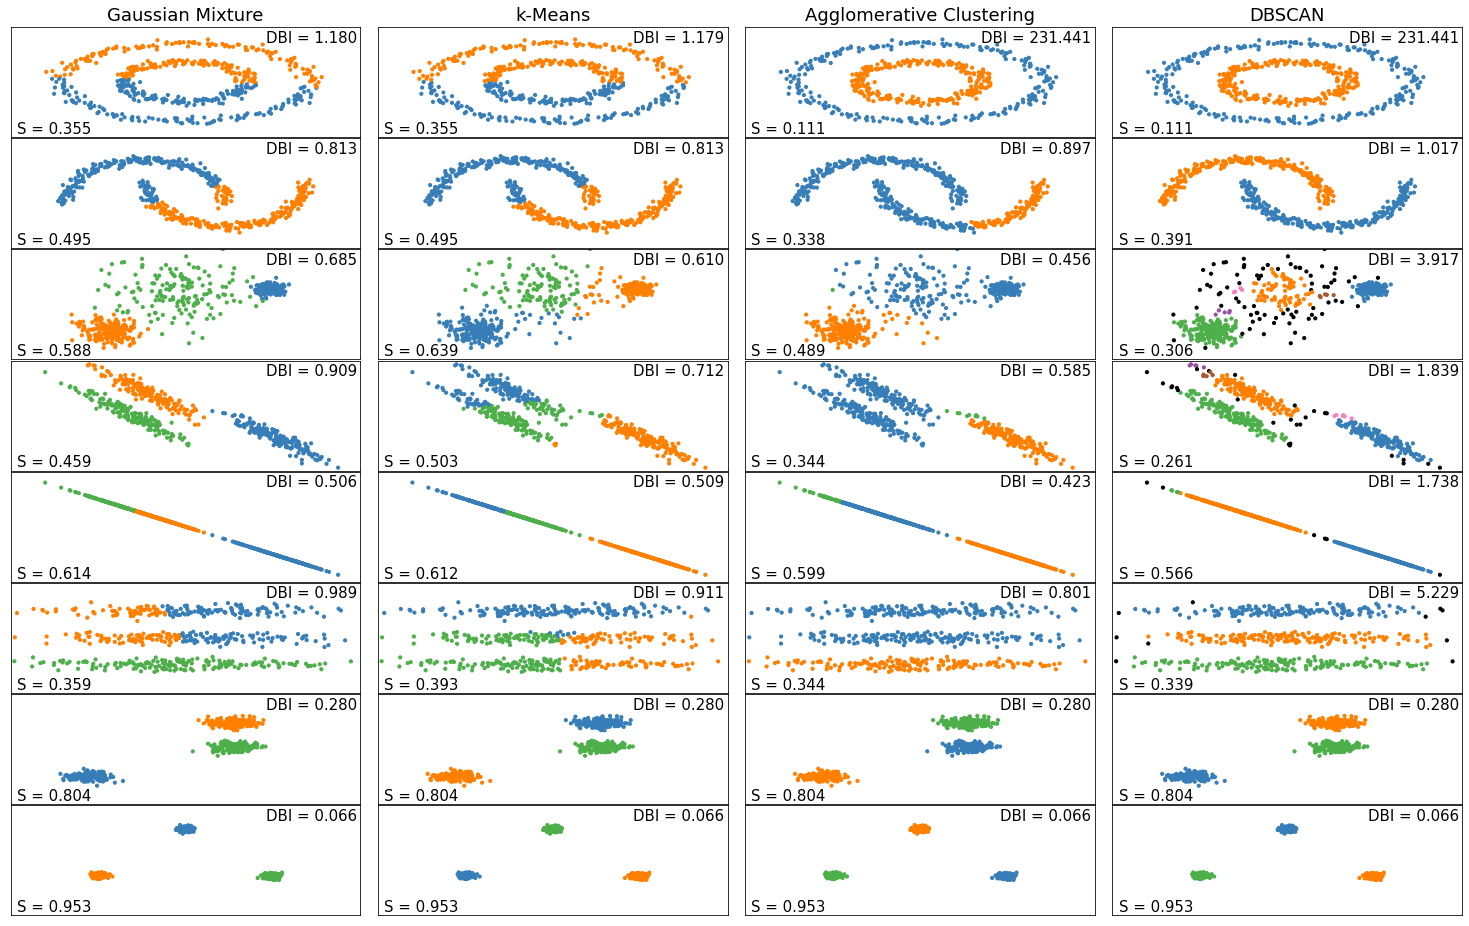
\includegraphics[scale = 0.3]{qual.png}
		\caption{Сравнение результатов работы различных алгоритмов кластеризации}
	\end{center}
\end{figure}


\section{Тематическое обучение  (Probabilistic LSA)}
\subsection{Идея}
\subsubsection*{Описание задачи тематического моделирования}

Тематическое моделирование --- технология статистического анализа текстов для автоматического выявления тематики в больших коллекциях документов

Тематическая модель --- модель коллекции текстовых документов, которая определяет, к каким темам относится каждый документ и какие слова (термины, термы) образуют каждую тему. Для этого не требуется никакой ручной разметки текстов, обучение модели происходит без учителя.

Чем-то похоже на кластеризацию, но тематическое моделирование в этом плане является «мягким» и допускает, чтобы документ относился к нескольким кластерам-темам. Тематическое моделирование не претендует на понимание смысла текста, однако оно способно отвечать на вопросы «о чём этот текст» или «какие общие темы имеет эта пара текстов».

Тематическая модель формирует сжатое векторное представление текста, которое помогает классифицировать, рубрицировать, аннотировать, сегментировать тексты. В отличие от известных векторных представлений семейства x2vec (word2vec, paragraph2vec, graph2vec и т.д.), в тематических векторах каждая координата соответствует теме и имеет содержательную интерпретацию. Модель привязывает к каждой теме список ключевых слов или фраз, который описывает семантику этой темы.

Тему нельзя строго определить ни семантически, ни эпистемологически. Темы выявляются исключительно с помощью автоматического подсчета правдоподобия совестной встречаемости слов. Слово может быть отнесено к нескольким темам, но с разной вероятностью, но слова-соседи для каждой темы у него будут разными. Высокочастотные служебные слова будут иметь примерно одинаковую вероятность для всех тем.

\subsubsection*{Зачем тематическое моделирование нужно:} 
\begin{itemize}
	\item разведочный информационный поиск (exploratory search) в электронных библиотеках;
	\item поиск по смыслу, а не по ключевым словам;
	\item обнаружение и отслеживание событий в новостных потоках;
	\item выявление тематических сообществ в социальных сетях;
	\item построение профилей интересов пользователей в рекомендательных системах;
	\item категоризация интентов в системах разговорного интеллекта;
	\item аннотирование изображений.
\end{itemize}

\subsubsection*{Параметры тематической модели }

\begin{itemize}
	\item $p(\omega | t)$  --- матрица искомых условных распределений слов по темам;
	\item $p(t | d)$ --- матрица искомых условных распределений тем по документам;
	\item $d$ --- документ;
	\item $\omega$ --- слово;
	\item $d,\omega$  --- наблюдаемые переменные;
	\item $t$  --- тема (скрытая переменная).
\end{itemize}

\begin{figure}[H]
	\begin{center}
		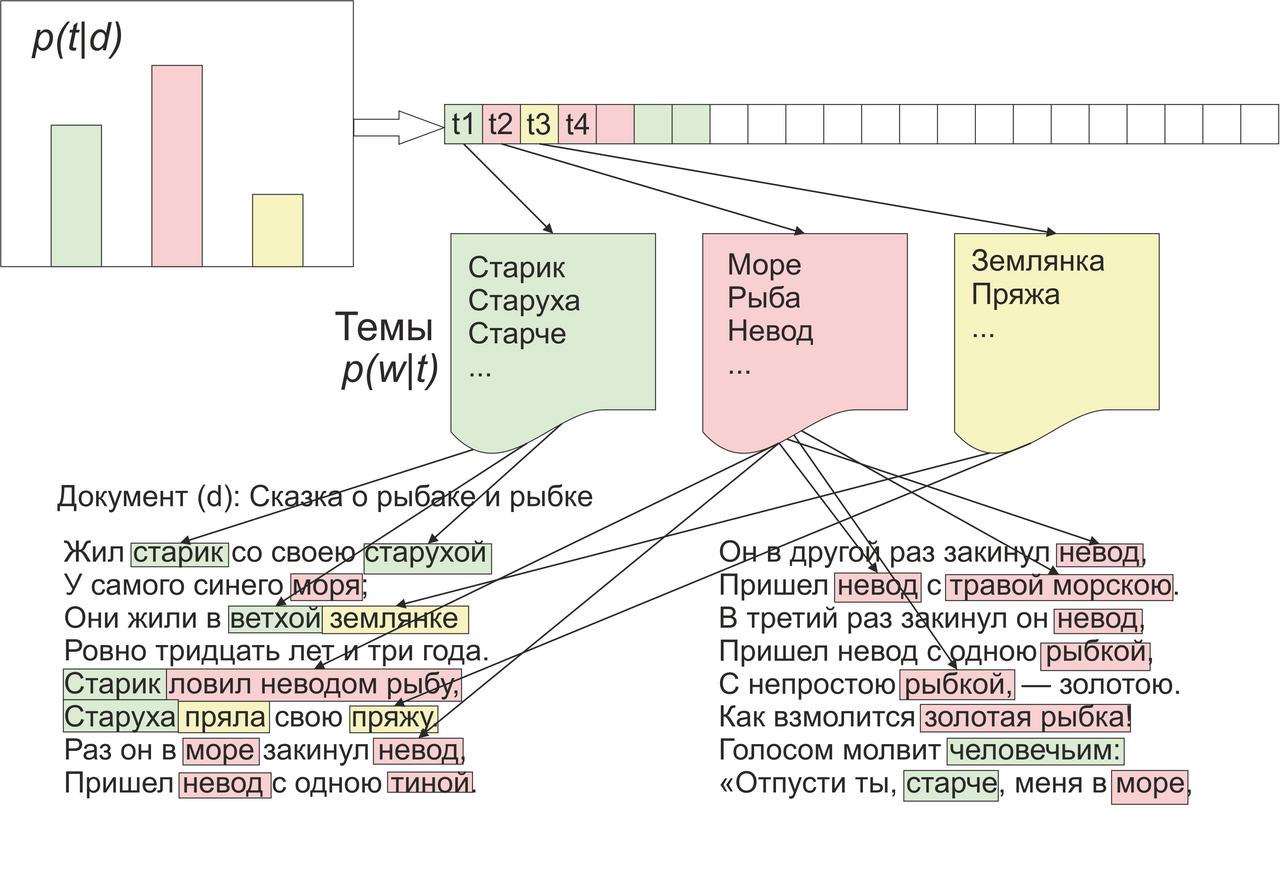
\includegraphics[scale = 1.5]{TM.png}
		\caption{Иллюстрация параметров модели тематического обучения.}
	\end{center}
\end{figure}

\subsection{LSA}

Латентно-семантический анализ, LSA (latent semantic analysis), он же LSI (latent semantic indexing) --- самая ранняя модель, предложенная еще в конце 80-х гг. Модель называется латентной, т.к. предполагает введение скрытого (латентного) параметра — темы.

LSA основан на использовании сингулярного разложения матрицы. С помощью SVD-разложения любая матрица раскладывается во множество ортогональных матриц, линейная комбинация которых является достаточно точным приближением к исходной матрице. Этим и объясняется название этого алгоритма в sklearn — TruncaredSVD.

\begin{figure}[H]
	\begin{center}
		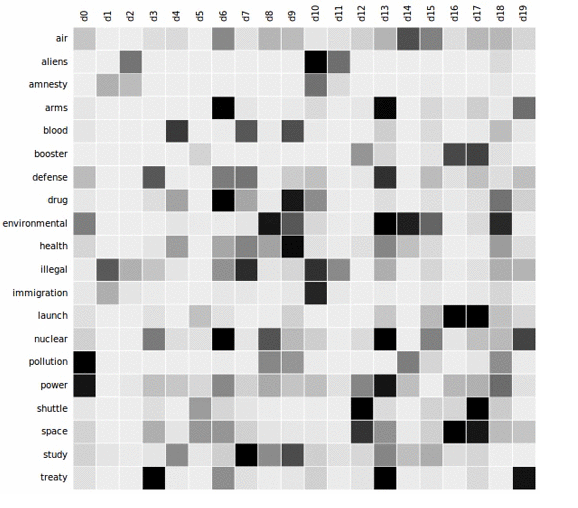
\includegraphics[scale = 0.5]{LSA1.png}
		\caption{Иллюстрация SVD в методе LSA (исходная матрица).}
	\end{center}
\end{figure}

\begin{figure}[H]
	\begin{center}
		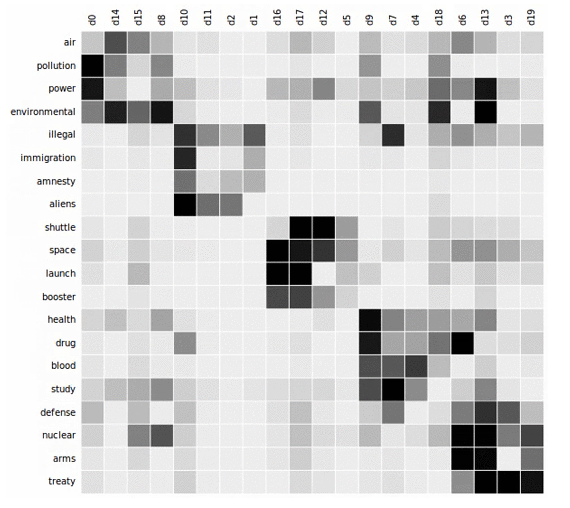
\includegraphics[scale = 0.5]{LSA2.png}
		\caption{Иллюстрация SVD в методе LSA.}
	\end{center}
\end{figure}

\subsection{Probabilistic LSA}

\subsubsection{Предпосылки появления}

pLSA (probabilistic latent semantic analysis), она же pLSI (probabilistic latent semantic indexing) --- вероятностный латентно-семантический анализ (индексирование). Модель предложена в 1999 г. Томасом Хоффманом.

Зачем понадобилось модифицировать LSA? Проблема этого метода в том, что он предполагает, что слова и документы имеют нормальное распределение, но в реальности это не так. Поэтому на практике чаще используется pLSA, основанный на мультиномиальном распределении. Если LSA — это чистая линейная алгебра, то pLSA имеет еще и статистические основания.

\subsubsection{Постановка задачи}

\textbf{Дана} коллекция текстовых документов (мешок слов): $n_{d\omega}$ --- сколько раз термин $\omega$ встречаетсяя в документе $d$.

\textbf{Найти} модель $p(\omega | d) = \sum_t \phi_{\omega t}\theta_{td}$ с параметрами $\phi, \theta$:

\begin{itemize}
	\item $\phi_{\omega t} = p(\omega | t)$  --- вероятности терминов $\omega$ в каждой теме $t$;
	\item $\theta_{td} = p(t | d)$ --- вероятности тем $t$ в каждом документе $d$.
\end{itemize}

\subsubsection{Обоснование решения}

Неизвестная модель находится путем максимизации логарифма правдоподобия:

$$ \sum_{d,\omega} n_{d,\omega} ln \sum_{t} \phi_{\omega t}\theta_{td} \rightarrow  \max_{\phi, \theta}$$

при ограничениях нормировки и неотрицательности:

$$ \phi_{\omega t} \geq 0; \sum_{\omega} \phi_{\omega t} = 1; \theta_{td} \geq 0; \sum_{t} \theta_{td} = 1$$

Точка максимума правдоподобия $\phi, \theta$ удовлетворяет системе уравнений со вспомогательными переменными $p_{td\omega}$:
$$
\begin{cases}
\displaystyle
p_{td\omega}={ {\phi_{\omega t} \theta_{td} } \over { \sum_{t'} \phi_{\omega t'} \theta_{t'd}}}\\
\phi_{\omega t} = { {n_{\omega t}} \over {\sum_{\omega `} n_{\omega `t}}}; n_{\omega t} = \sum_{d \in D} n_{d\omega}p_{td\omega}\\
\theta_{td} = { {n_{td}} \over {\sum_{t'}n_{t'd}}}; n_{td} = \sum_{\omega \in d} n_{d\omega}p_{td\omega}
\end{cases}
$$

Где первое уравнение это $E$-шаг $EM$ алгоритма, а второе и третье уравнение --- $M$-шаг.

\subsubsection*{$E$-шаг -- это формула Байеса:}

$$p_{td\omega} = p(t | d, \omega) = { {p(\omega , t | d)} \over {p(\omega | d)}} = { {p(\omega | t) p(t|d)} \over {p(\omega | d)}}= {{\phi_{\omega t}\theta_{td}} \over {\sum_{s \in T}\phi_{\omega t}\theta_{td}}}$$

$n_{d \omega t} = n_{d \omega}p(t | d, \omega)$ --- оценка числа троек $(d, \omega, t)$ в коллекции


\subsubsection*{$M$-шаг --- это частотные оценки условных вероятностей:}

$$ \phi_{\omega t} = {{n_{\omega t}} \over {n_t}} \equiv {{\sum_{d \in D} n_{d \omega t}} \over {\sum_{d \in D} \sum_{\omega \in d} n_{d \omega t}}} $$

$$ \theta_{td} = { {n_td} \over {n_d}} \equiv {{\sum_{\omega \in D} n_{d \omega t}} \over {\sum_{\omega \in \Omega} \sum_{t \in T} n_{d \omega t}}}$$

\newpage
\subsubsection{EM-алгоритм}

Описание EM-алгоритма:

\textbf{Вход:} коллекция $D$, число тем $|T|$ и число иттераций $i_{max}$;
	
\textbf{Выход:} матрица терминов тем $\Theta$ и тем документов $\Phi$;

\begin{enumerate}
		\item инициализация $\phi_{\omega t}, \theta_{td}$ для всех $d \in D, \omega \in \Omega, t \in T$; 
		\item \textbf{для всех} иттераций $i=1, \cdots, i_{max}$ 
		\item \quad $n_{\omega t}, n_{td}, n_t, n_d := 0$ для всех $d \in D, \omega \in \Omega, t \in T$; 
		\item \quad \textbf{для всех} документов  $d \in D$ и слов $\omega \in d$
		\item \quad \quad $p_{td\omega} = {{\phi_{\omega t} \theta_{td}} \over {\sum_{s} \phi_{\omega s} \theta_{sd}}}$; 
		\item \quad \quad $n_{\omega t}, n_{td}, n_t, n_d += n_{d \omega} p_{td \omega}$ для всех $t \in T$;
		\item \quad $\phi_{\omega t} := n_{\omega t}/n_t$ для всех $\omega \in \Omega, t \in T$;
		\item \quad $\phi_{td} := n_{td}/n_d$ для всех $d \in D, t \in T$;

\end{enumerate}

\end{document}
